\documentclass{standalone}
\usepackage{tikz}
\usetikzlibrary{patterns, positioning}


\begin{document}
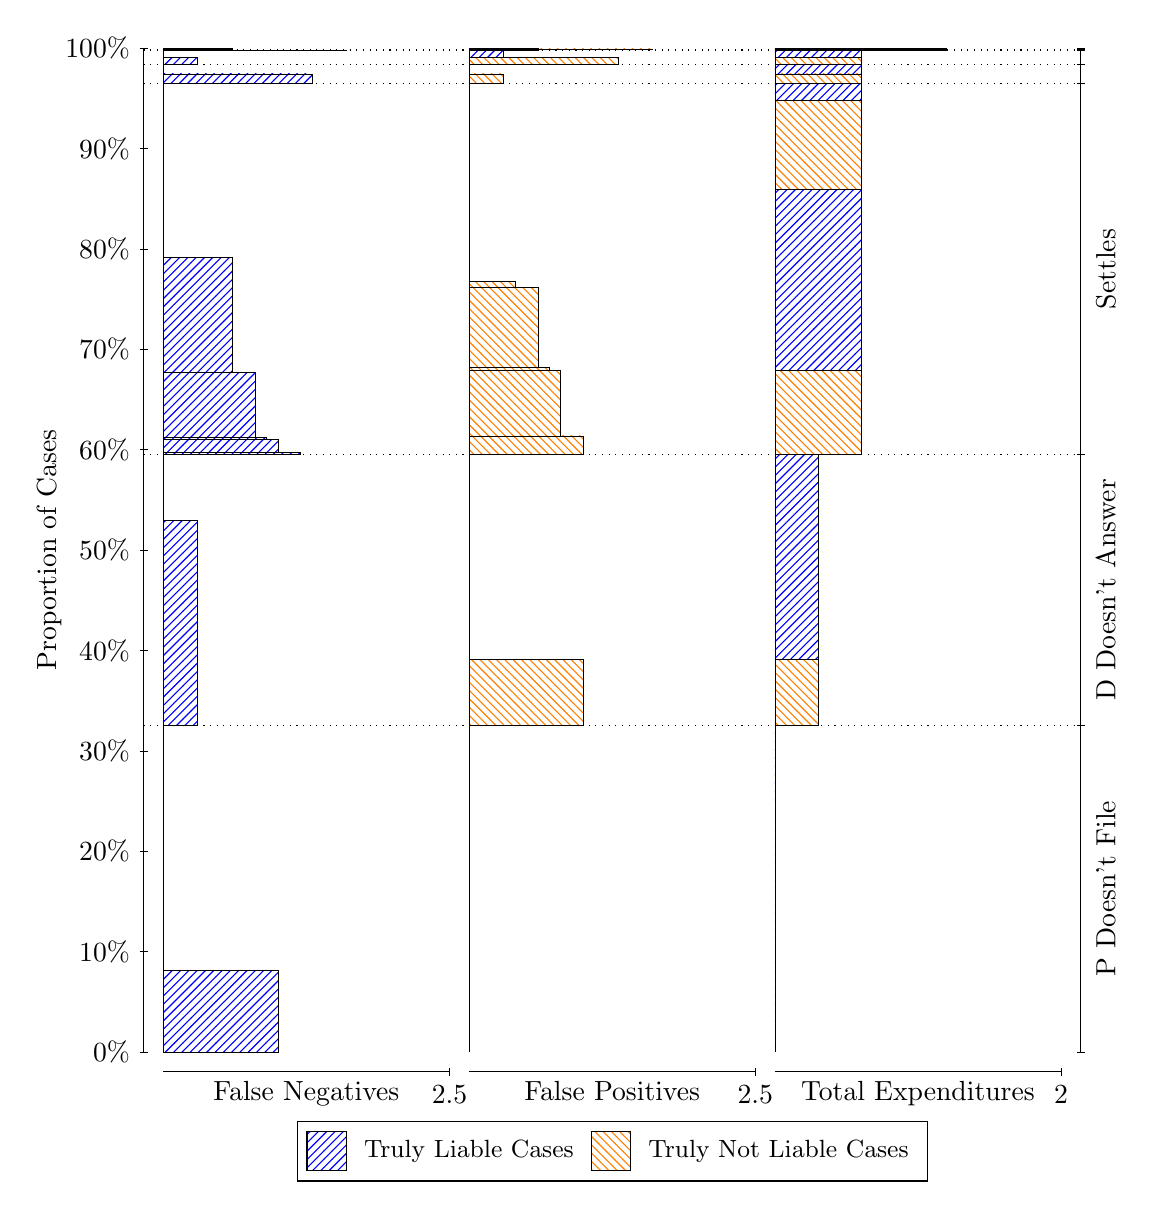
\begin{tikzpicture}
\draw[black, very thin] (1.5,1.75) -- (1.5,14.5);
\node[rotate=90, text=black, anchor=center] at (0.3, 8.125) {Proportion of Cases};
\draw[black, very thin] (1.45,1.75) -- (1.55,1.75);
\node[text=black, anchor=east] at (1.45, 1.75) {0\%};
\draw[black, very thin] (1.45,3.025) -- (1.55,3.025);
\node[text=black, anchor=east] at (1.45, 3.025) {10\%};
\draw[black, very thin] (1.45,4.3) -- (1.55,4.3);
\node[text=black, anchor=east] at (1.45, 4.3) {20\%};
\draw[black, very thin] (1.45,5.575) -- (1.55,5.575);
\node[text=black, anchor=east] at (1.45, 5.575) {30\%};
\draw[black, very thin] (1.45,6.85) -- (1.55,6.85);
\node[text=black, anchor=east] at (1.45, 6.85) {40\%};
\draw[black, very thin] (1.45,8.125) -- (1.55,8.125);
\node[text=black, anchor=east] at (1.45, 8.125) {50\%};
\draw[black, very thin] (1.45,9.4) -- (1.55,9.4);
\node[text=black, anchor=east] at (1.45, 9.4) {60\%};
\draw[black, very thin] (1.45,10.675) -- (1.55,10.675);
\node[text=black, anchor=east] at (1.45, 10.675) {70\%};
\draw[black, very thin] (1.45,11.95) -- (1.55,11.95);
\node[text=black, anchor=east] at (1.45, 11.95) {80\%};
\draw[black, very thin] (1.45,13.225) -- (1.55,13.225);
\node[text=black, anchor=east] at (1.45, 13.225) {90\%};
\draw[black, very thin] (1.45,14.5) -- (1.55,14.5);
\node[text=black, anchor=east] at (1.45, 14.5) {100\%};

\draw[black, very thin] (13.4,1.75) -- (13.4,14.5);
\draw[black, very thin] (13.35,1.75) -- (13.45,1.75);
\node[anchor=west] at (13.35, 1.75) {};
\draw[black, very thin] (13.35,5.8963) -- (13.45,5.8963);
\node[anchor=west] at (13.35, 5.8963) {};
\draw[black, very thin] (13.35,9.3387) -- (13.45,9.3387);
\node[anchor=west] at (13.35, 9.3387) {};
\draw[black, very thin] (13.35,14.047) -- (13.45,14.047);
\node[anchor=west] at (13.35, 14.047) {};
\draw[black, very thin] (13.35,14.296) -- (13.45,14.296);
\node[anchor=west] at (13.35, 14.296) {};
\draw[black, very thin] (13.35,14.468) -- (13.45,14.468);
\node[anchor=west] at (13.35, 14.468) {};
\draw[black, very thin] (13.35,14.483) -- (13.45,14.483);
\node[anchor=west] at (13.35, 14.483) {};
\draw[black, very thin] (13.35,14.5) -- (13.45,14.5);
\node[anchor=west] at (13.35, 14.5) {};

\draw[black, very thin, pattern color=blue, pattern=north east lines] (1.75,1.75) rectangle (3.2033,2.782);
\draw[black, very thin, pattern color=orange, pattern=north west lines] (1.75,2.782) rectangle (1.75,5.8963);
\draw[black, very thin, pattern color=blue, pattern=north east lines] (1.75,5.8963) rectangle (2.186,8.5025);
\draw[black, very thin, pattern color=orange, pattern=north west lines] (1.75,8.5025) rectangle (1.75,9.3387);
\draw[black, very thin, pattern color=blue, pattern=north east lines] (1.75,9.3387) rectangle (3.494,9.361);
\draw[black, very thin, pattern color=blue, pattern=north east lines] (1.75,9.361) rectangle (3.2033,9.5334);
\draw[black, very thin, pattern color=blue, pattern=north east lines] (1.75,9.5334) rectangle (3.058,9.5539);
\draw[black, very thin, pattern color=blue, pattern=north east lines] (1.75,9.5539) rectangle (2.9127,10.385);
\draw[black, very thin, pattern color=blue, pattern=north east lines] (1.75,10.385) rectangle (2.622,11.846);
\draw[black, very thin, pattern color=orange, pattern=north west lines] (1.75,11.846) rectangle (1.75,14.047);
\draw[black, very thin, pattern color=blue, pattern=north east lines] (1.75,14.047) rectangle (3.6393,14.172);
\draw[black, very thin, pattern color=orange, pattern=north west lines] (1.75,14.172) rectangle (1.75,14.296);
\draw[black, very thin, pattern color=blue, pattern=north east lines] (1.75,14.296) rectangle (2.186,14.383);
\draw[black, very thin, pattern color=orange, pattern=north west lines] (1.75,14.383) rectangle (1.75,14.468);
\draw[black, very thin, pattern color=blue, pattern=north east lines] (1.75,14.468) rectangle (4.0753,14.473);
\draw[black, very thin, pattern color=orange, pattern=north west lines] (1.75,14.473) rectangle (1.75,14.483);
\draw[black, very thin, pattern color=blue, pattern=north east lines] (1.75,14.483) rectangle (2.622,14.495);
\draw[black, very thin, pattern color=orange, pattern=north west lines] (1.75,14.495) rectangle (1.75,14.5);
\draw[black, very thin, pattern color=orange, pattern=north west lines] (5.6333,1.75) rectangle (5.6333,4.8642);
\draw[black, very thin, pattern color=blue, pattern=north east lines] (5.6333,4.8642) rectangle (5.6333,5.8963);
\draw[black, very thin, pattern color=orange, pattern=north west lines] (5.6333,5.8963) rectangle (7.0867,6.7325);
\draw[black, very thin, pattern color=blue, pattern=north east lines] (5.6333,6.7325) rectangle (5.6333,9.3387);
\draw[black, very thin, pattern color=orange, pattern=north west lines] (5.6333,9.3387) rectangle (7.0867,9.5733);
\draw[black, very thin, pattern color=orange, pattern=north west lines] (5.6333,9.5733) rectangle (6.796,10.408);
\draw[black, very thin, pattern color=orange, pattern=north west lines] (5.6333,10.408) rectangle (6.6507,10.448);
\draw[black, very thin, pattern color=orange, pattern=north west lines] (5.6333,10.448) rectangle (6.5053,11.458);
\draw[black, very thin, pattern color=orange, pattern=north west lines] (5.6333,11.458) rectangle (6.2147,11.54);
\draw[black, very thin, pattern color=blue, pattern=north east lines] (5.6333,11.54) rectangle (5.6333,14.047);
\draw[black, very thin, pattern color=orange, pattern=north west lines] (5.6333,14.047) rectangle (6.0693,14.171);
\draw[black, very thin, pattern color=blue, pattern=north east lines] (5.6333,14.171) rectangle (5.6333,14.296);
\draw[black, very thin, pattern color=orange, pattern=north west lines] (5.6333,14.296) rectangle (7.5227,14.381);
\draw[black, very thin, pattern color=blue, pattern=north east lines] (5.6333,14.381) rectangle (6.0693,14.468);
\draw[black, very thin, pattern color=orange, pattern=north west lines] (5.6333,14.468) rectangle (6.5053,14.478);
\draw[black, very thin, pattern color=blue, pattern=north east lines] (5.6333,14.478) rectangle (5.6333,14.483);
\draw[black, very thin, pattern color=orange, pattern=north west lines] (5.6333,14.483) rectangle (7.9587,14.488);
\draw[black, very thin, pattern color=blue, pattern=north east lines] (5.6333,14.488) rectangle (6.5053,14.5);
\draw[black, very thin, pattern color=orange, pattern=north west lines] (9.5167,1.75) rectangle (9.5167,4.8642);
\draw[black, very thin, pattern color=blue, pattern=north east lines] (9.5167,4.8642) rectangle (9.5167,5.8963);
\draw[black, very thin, pattern color=orange, pattern=north west lines] (9.5167,5.8963) rectangle (10.062,6.7325);
\draw[black, very thin, pattern color=blue, pattern=north east lines] (9.5167,6.7325) rectangle (10.062,9.3387);
\draw[black, very thin, pattern color=orange, pattern=north west lines] (9.5167,9.3387) rectangle (10.607,10.408);
\draw[black, very thin, pattern color=blue, pattern=north east lines] (9.5167,10.408) rectangle (10.607,12.7);
\draw[black, very thin, pattern color=orange, pattern=north west lines] (9.5167,12.7) rectangle (10.607,13.832);
\draw[black, very thin, pattern color=blue, pattern=north east lines] (9.5167,13.832) rectangle (10.607,14.047);
\draw[black, very thin, pattern color=orange, pattern=north west lines] (9.5167,14.047) rectangle (10.607,14.171);
\draw[black, very thin, pattern color=blue, pattern=north east lines] (9.5167,14.171) rectangle (10.607,14.296);
\draw[black, very thin, pattern color=orange, pattern=north west lines] (9.5167,14.296) rectangle (10.607,14.381);
\draw[black, very thin, pattern color=blue, pattern=north east lines] (9.5167,14.381) rectangle (10.607,14.468);
\draw[black, very thin, pattern color=orange, pattern=north west lines] (9.5167,14.468) rectangle (11.697,14.478);
\draw[black, very thin, pattern color=blue, pattern=north east lines] (9.5167,14.478) rectangle (11.697,14.483);
\draw[black, very thin, pattern color=orange, pattern=north west lines] (9.5167,14.483) rectangle (11.697,14.488);
\draw[black, very thin, pattern color=blue, pattern=north east lines] (9.5167,14.488) rectangle (11.697,14.5);
\draw[black, dotted] (1.5,5.8963) -- (13.4,5.8963);
\draw[black, dotted] (1.5,9.3387) -- (13.4,9.3387);
\draw[black, dotted] (1.5,14.047) -- (13.4,14.047);
\draw[black, dotted] (1.5,14.296) -- (13.4,14.296);
\draw[black, dotted] (1.5,14.468) -- (13.4,14.468);
\draw[black, dotted] (1.5,14.483) -- (13.4,14.483);
\draw[black, very thin] (1.75,1.5) -- (5.3833,1.5);
\node[text=black, anchor=north] at (3.5667, 1.5) {False Negatives};
\draw[black, very thin] (5.3833,1.45) -- (5.3833,1.55);
\node[text=black, anchor=north] at (5.3833, 1.45) {2.5};

\draw[black, very thin] (5.6333,1.5) -- (9.2667,1.5);
\node[text=black, anchor=north] at (7.45, 1.5) {False Positives};
\draw[black, very thin] (9.2667,1.45) -- (9.2667,1.55);
\node[text=black, anchor=north] at (9.2667, 1.45) {2.5};

\draw[black, very thin] (9.5167,1.5) -- (13.15,1.5);
\node[text=black, anchor=north] at (11.333, 1.5) {Total Expenditures};
\draw[black, very thin] (13.15,1.45) -- (13.15,1.55);
\node[text=black, anchor=north] at (13.15, 1.45) {2};

\node[text=black, centered, rotate=90] at (13.72, 3.8231) {P Doesn't File};
\node[text=black, centered, rotate=90] at (13.72, 7.6175) {D Doesn't Answer};
\node[text=black, centered, rotate=90] at (13.72, 11.693) {Settles};





\draw (7.449999999999999,1.5) node[draw=none] (baseCoordinate) {};
\begin{scope}[align=center]
        \matrix[scale=0.5, draw=black, below=0.5cm of baseCoordinate, nodes={draw}, column sep=0.1cm]{
            \node[rectangle, draw, minimum width=0.5cm, minimum height=0.5cm, pattern color=blue, pattern=north east lines] {}; &
            \node[draw=none, font=\small, text=black] (B) {Truly Liable Cases}; &
            \node[rectangle, draw, minimum width=0.5cm, minimum height=0.5cm, pattern color=orange, pattern=north west lines] {}; &
            \node[draw=none, font=\small, text=black] (B) {Truly Not Liable Cases}; \\
            };
\end{scope}

\end{tikzpicture}
\end{document}